% Figure 2, generated by analyze.py: accuracy in % of the ridge accuracy (mean over the 10 benchmarks, bars = interquartile range)
% vs training energy relative to the ridge readout (geometric mean; WiSARD readouts with hashed RAM nodes of 256 counters).
\definecolor{cRidge}{HTML}{2A78D6}\definecolor{cRq}{HTML}{EB6834}\definecolor{cWMM}{HTML}{1BAF7A}\definecolor{cWQU}{HTML}{EDA100}\definecolor{cWQG}{HTML}{E87BA4}
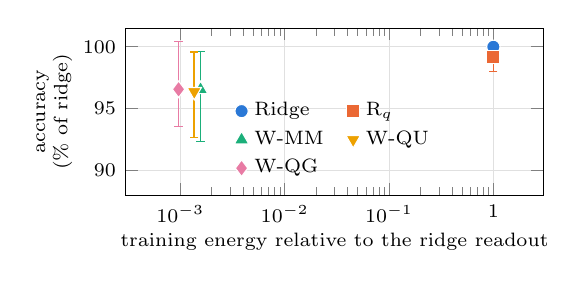
\begin{tikzpicture}
\begin{axis}[width=5.3cm, height=2.12cm, scale only axis, xmode=log, xmin=3e-4, xmax=3, ymin=88, ymax=101.5,
  xtick={0.001,0.01,0.1,1}, xticklabels={$10^{-3}$,$10^{-2}$,$10^{-1}$,$1$}, ytick={90,95,100},
  xlabel={training energy relative to the ridge readout}, ylabel={accuracy\\(\% of ridge)}, ylabel style={align=center},
  label style={font=\scriptsize}, tick label style={font=\scriptsize}, xlabel shift=-3pt, ylabel shift=-3pt,
  grid=major, grid style={line width=0.3pt, draw=black!12}, axis line style={line width=0.4pt},
  legend style={font=\scriptsize, draw=none, fill=none, at={(0.5,0.04)}, anchor=south, legend columns=2, /tikz/every even column/.append style={column sep=6pt}},
  legend cell align=left]
\addplot[only marks, color=cRidge, mark=*, mark options={fill=cRidge, draw=white, line width=0.4pt, mark size=2.4pt}] coordinates {(1.0, 100.0)};
\addlegendentry{Ridge}
\addplot[only marks, color=cRq, mark=square*, mark options={fill=cRq, draw=white, line width=0.4pt, mark size=2.4pt}, error bars/.cd, y dir=both, y explicit, error bar style={line width=0.6pt, color=cRq}, error mark options={rotate=90, mark size=1.5pt, color=cRq}] coordinates {(1, 99.15) -= (0, 1.16) += (0, 1.20)};
\addlegendentry{R$_q$}
\addplot[only marks, color=cWMM, mark=triangle*, mark options={fill=cWMM, draw=white, line width=0.4pt, mark size=3pt}, error bars/.cd, y dir=both, y explicit, error bar style={line width=0.6pt, color=cWMM}, error mark options={rotate=90, mark size=1.5pt, color=cWMM}] coordinates {(0.001563, 96.55) -= (0, 4.19) += (0, 3.10)};
\addlegendentry{W-MM}
\addplot[only marks, color=cWQU, mark=triangle*, mark options={fill=cWQU, draw=white, line width=0.4pt, mark size=3pt, rotate=180}, error bars/.cd, y dir=both, y explicit, error bar style={line width=0.6pt, color=cWQU}, error mark options={rotate=90, mark size=1.5pt, color=cWQU}] coordinates {(0.00136, 96.37) -= (0, 3.73) += (0, 3.21)};
\addlegendentry{W-QU}
\addplot[only marks, color=cWQG, mark=diamond*, mark options={fill=cWQG, draw=white, line width=0.4pt, mark size=3pt}, error bars/.cd, y dir=both, y explicit, error bar style={line width=0.6pt, color=cWQG}, error mark options={rotate=90, mark size=1.5pt, color=cWQG}] coordinates {(0.000962, 96.56) -= (0, 3.01) += (0, 3.86)};
\addlegendentry{W-QG}
\end{axis}
\end{tikzpicture}
